\documentclass[tikz,border=2pt]{standalone}
\usepackage{mathptmx}
\usepackage{amsmath}
\usetikzlibrary{arrows.meta,calc}
\definecolor{pvblue}{HTML}{0072B2}
\definecolor{pvorange}{HTML}{D55E00}
\definecolor{pvink}{HTML}{374151}
\definecolor{pvmuted}{HTML}{9AA5B1}
\begin{document}
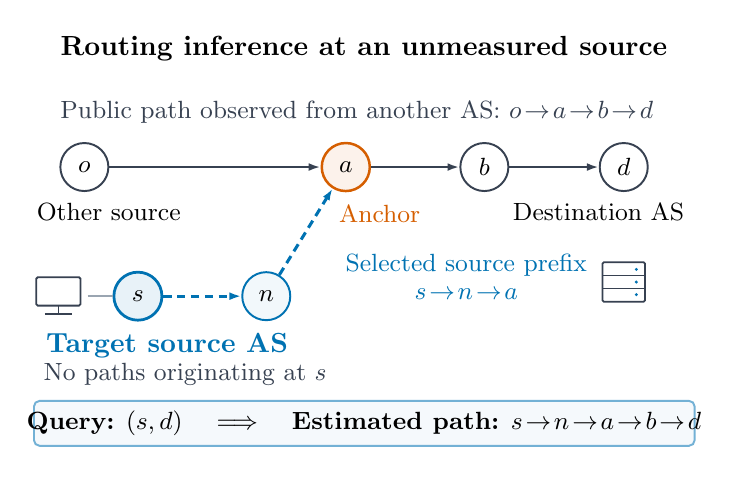
\begin{tikzpicture}[
 font=\fontsize{8.8}{10.1}\selectfont,
 >={Latex[length=1.5mm,width=1mm]},
 as/.style={circle,draw=pvink,fill=white,line width=.7pt,
  minimum size=.61cm,inner sep=0pt},
 label/.style={align=center,inner sep=0pt},
 prefixedge/.style={->,pvblue,line width=1.1pt,dash pattern=on 3pt off 2pt},
 observededge/.style={->,pvink,line width=1.0pt}
]
\path[use as bounding box] (0,0) rectangle (8.55,5.35);
\node[font=\bfseries\fontsize{10}{11.2}\selectfont] at (4.27,5.08)
 {Routing inference at an unmeasured source};

% A measured route originates elsewhere; its tail can be reused.
\node[as] (o) at (.72,3.58) {$o$};
\node[as,draw=pvorange,fill=pvorange!8,line width=.9pt] (a) at (4.04,3.58) {$a$};
\node[as] (b) at (5.80,3.58) {$b$};
\node[as] (d) at (7.57,3.58) {$d$};
\draw[observededge] (o)--(a);
\draw[observededge] (a)--(b);
\draw[observededge] (b)--(d);
\node[label,text=pvink] at (4.18,4.28) {Public path observed from another AS: $o\!\to\!a\!\to\!b\!\to\!d$};
\node[label,anchor=north] at (1.03,3.13) {Other source};
\node[label,text=pvorange,anchor=north] at (4.47,3.10) {Anchor};
\node[label,anchor=north] at (7.25,3.13) {Destination AS};

% The selected prefix joins the public route at its anchor.
\node[as,draw=pvblue,fill=pvblue!9,line width=1pt] (s) at (1.40,1.94) {$s$};
\node[as,draw=pvblue,fill=pvblue!5] (n) at (3.03,1.94) {$n$};
\draw[prefixedge] (s)--(n);
\draw[prefixedge] (n)--(a);
\node[label,text=pvblue] at (5.57,2.18) {Selected source prefix\\$s\!\to\!n\!\to\!a$};
\node[label,text=pvblue,anchor=north,font=\bfseries] at (1.77,1.47) {Target source AS};
\node[label,text=pvink] at (2.00,.95) {No paths originating at $s$};

% Small monitor/server icons connect the AS task to network applications.
\begin{scope}[shift={(.39,1.99)}]
 \draw[pvink,line width=.65pt,rounded corners=.5pt] (-.28,-.17) rectangle (.28,.19);
 \draw[pvink,line width=.6pt] (0,-.17)--(0,-.28) (-.17,-.28)--(.17,-.28);
\end{scope}
\draw[pvmuted,line width=.6pt] (.76,1.94)--(s.west);
\begin{scope}[shift={(7.57,2.12)}]
 \draw[pvink,line width=.65pt,rounded corners=.5pt] (-.27,-.25) rectangle (.27,.25);
 \draw[pvink,line width=.55pt] (-.27,.08)--(.27,.08) (-.27,-.08)--(.27,-.08);
 \foreach \y in {-.16,0,.16} {\fill[pvblue] (.16,\y) circle (.021);}
\end{scope}


\draw[rounded corners=2pt,draw=pvblue!55,fill=pvblue!4,line width=.7pt]
 (.08,.04) rectangle (8.47,.61);
\node[label] at (4.27,.33) {\textbf{Query:} $(s,d)$ \quad $\Longrightarrow$ \quad \textbf{Estimated path:} $s\!\to\!n\!\to\!a\!\to\!b\!\to\!d$};
\end{tikzpicture}
\end{document}
